\chapter{Towards a general model for shallow magmatic intrusions}
\label{chap7}

\section{Summary}
\label{sec:summary-2}

\citet{Michaut:2011kg} originally provides a model which describes the
dynamics  of shallow  magmatic  intrusions.  In particular,  depending
mainly  on the  injection  rate  and the  intrusion  depth, the  model
predicts  two   regimes  of  propagation  characterized   by  specific
morphologies and  scaling laws  for intrusion thickness  versus length
and  time.  This model  predicts  the  appropriate geometry  for  both
terrestrial  laccoliths and  large mafic  sills. However,  we show  in
Chapter \ref{chap2} that it  underestimates the absolute dimensions of
these magmatic intrusions; in  particular, it requires abnormally high
viscosity to reconcile both observations and predictions.

To get  some insights in the  effective flow viscosity, we  develop in
chapter \ref{C3-JFM}  and \ref{Heating} an  extension of the  model of
\citet{Michaut:2011kg} that  accounts for the cooling  of the current.
We show that  the coupling between the temperature field  and the flow
itself leads  to the formation of  a highly viscous region  at the tip
which slows  down the  spreading in both  regimes. The  intrusions are
predicted  to  be thicker  and  their  dimensions, especially  in  the
bending regime, are now consistent with the observations.

In Chapter  \ref{C5-chap6}, we  neglect the  cooling to  relax another
assumption of  the original model of  \citet{Michaut:2011kg}, i.e. the
constant thickness  of the  upper layer. In  particular, we  study the
effect of a crater depression located on top of the intrusion. We show
that  the  lithostatic barrier  imposed  by  the  crater wall  at  the
periphery of  the depression prevents  the spreading of  the intrusion
which  instead  thickens. This  second  model  also shows  predictions
consistent with the deformations observed at floor-fractured craters.

Promising  comparison between  predictions  and  observations such  as
these  should  drive a  methodical  and  rigorous improvement  of  the
mathematical model for the emplacement of shallow magmatic intrusions.
Nevertheless,  we also  show the  limit of  using field  observations,
whose  parameters  are  poorly  constrained,  to  validate  the  model
predictions.   An  alternative  approach  could  be  to  use  analogue
experiments that are  designed to produce some feature  of the natural
system at a  laboratory scale. Indeed, such  experiments could provide
useful   benchmarks  for   the   theoretical   model.   In   addition,
phenomenological observations not predicted  by the theory could guide
further investigations  towards our  understanding of  shallow magmatic
intrusions.

\section{What does limit the extent of magmatic intrusions?}
\label{sec:summary-2}

While  the crater  depression clearly  limits the  flow expansion  for
crater-centered intrusions,  one can  wonder about why  laccoliths and
sills stop  their propagation  in the third  bending phase  and second
gravity phase respectively. Available  data on terrestrial laccoliths,
used in combination  with the model, show  that terrestrial laccoliths
probably do  not stop  following the formation  of the  highly viscous
region  at  the  intrusion  front,  as  initially  suggested  (Section
\ref{Heating}).

Instead, a  tempting hypothesis  is that the  limited volume  of magma
initially   available    simply   limits    the   extent    of   these
intrusions. Indeed, one  may expect that the injection  rate, which is
considered constant in this model, wanes as the deep magma source gets
exhausted.  Depending  on the  local  emplacement  conditions, if  the
injection rate lasts sufficiently long for the intrusion to transition
to the  gravity regime,  the intrusion  solidifies as  a sill.  In the
contrary,  the  intrusion  solidifies  as  a  laccolith.  The  current
thickness and  time at  the transition depend  on the  composition. In
particular, the  more evolved  the magma  composition, the  larger the
transition time and the larger  the volume required for the transition
to  occur.  Together,  it   corroborates  the  predominance  in  field
observations of felsic laccoliths and mafic sills.

In  addition, in  chapter \ref{Heating},  we show  that a  significant
thermal aureole  should develop  in the wall  rocks above  the central
flow region. Apart from plastic rock deformation that might develop in
the overburden, the  thermal erosion above the feeder  dyke, where the
temperature are  expected to be  maximum, might also  favor subsequent
dyke propagation and limit the size  of the intrusion. This could also
potentially  explain   the  nested  structure  of   several  laccolith
complexes reported in the literature \citep{E:2015tl,Rocchi:2010dn}.

Alternatively, fracturation  at the  front could  limit the  extent of
some magmatic intrusions and trigger  their arrest. Indeed, for a sake
of simplicity, we used a thin prewetting  film at the tip to avoid the
requirement of any boundary condition at a genuine front in the models
developed in this thesis.  Nevertheless, a necessary extension of this
work  is the  description of  a  realistic boundary  condition at  the
intrusion front which includes a realistic fracturation criterion.

\section{Rigorous treatment of the front}
\label{sec:rigor-treatm-front}

\subsubsection*{Fracturation}
\label{sec:fracturation}

A first step  would be to describe  the tip in term of  a fluid driven
fracture  instead of  the thin  prewetting  film. As  seen in  Section
\ref{C2-Toughness},  linear elastic  fracture mechanics  requires that
the  mode $I$  intensity factor  $K_I$  equals a  critical value,  the
fracture toughness  of the wall  rock $K_{c}$, for the  propagation to
occur. This  condition is usually  expressed in term of  an asymptotic
condition    on    the    crack     opening    $h(r,t)$    at    $r=R$
\citep{Savitski:2002gy,Bunger:2005em,Bunger:2007vs,Detournay:2014fk}.

In  such  problem,  the  thickness  equation  is  thus  coupled  to  a
description  of  the fracture  opening  based  on the  linear  elastic
fracture mechanics. \citet{Bunger:2011cb} used  this approach to solve
the  problem  of  isoviscous  shallow magmatic  intrusions  and  found
similar  results  than   \citet{Michaut:2011kg}.  Interestingly,  they
needed values for the fracture toughness  $K_c$ two or three orders of
magnitudes  larger  than  laboratory  measurements  to  reproduce  the
observations.  In  addition, they  found  that  the apparent  fracture
toughness of  laccoliths is  much larger than  for large  mafic sills,
which they  attribute to potentially  crack blunting mechanism  at the
tip  of laccoliths.  This  observation is  consistent  with the  rapid
formation  of  a highly  viscous  plug  at  the  tip of  the  magmatic
intrusion described in Chapter \ref{C3-JFM} and \ref{Heating}.

Nevertheless, this model also falls short to reproduce the behavior of
large  mafic sills.   In addition,  more realistic  model should  also
consider the process zone, i.e. the region of plastic rock deformation
near the leading edge of the fracture \citep{Bunger:2008cl}. Moreover,
the large  negative pressure that  developed at the front  might cause
dissolved gasses to exsolve from the magma \citep{Lister:2013ia}. With
the formation and the evolution of a gap filled with gas at the tip of
the current, the fluid and the fracture front do not coincide with one
another, thus requiring the tracking of two moving boundaries.

\subsubsection*{Fluid gap}
\label{sec:fracturation}

Along      with      the     prewetting      film      regularization,
\citet{Anonymous:QWXp_4JV} propose  a second  regularization condition
where the tip of the elastic-plated  gravity current consists of a lag
region  filled  with  gas  at a  constant  negative  pressure  (Figure
\ref{C7-Sketch}).   They show  that the  solution depends  on the  gas
pressure in  the tip  region in  a similar  fashion that  the solution
depends  on  the prewetting  film  thickness  in Chapter  \ref{chap2},
\ref{C3-JFM} and \ref{Heating}.
\begin{figure}[h!]
 \begin{center}
 \graphicspath{ {/Users/thorey/Documents/These/Manuscript/Figure/Chapter7/} }
 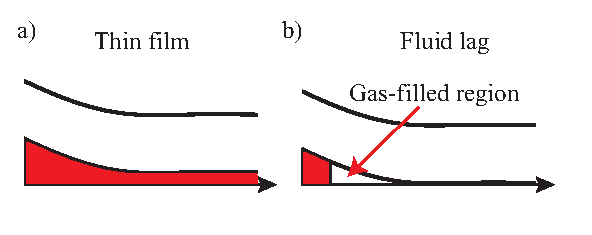
\includegraphics[scale=1.3]{Sketch.eps}
 \caption{Two different regularization condition at the front of
 the current: a) thin prewetting film with thickness $h_f$ b) gas
 -filled region.}
 \label{C7-Sketch}
 \end{center}
\end{figure}
In particular, in a Cartesian geometry, they show that
\begin{eqnarray}
 h_0&\propto& h_f^{-1/7}\nu^{-2/7}L^{10/7}~(\text{Thin film})\\
 h_0&\propto& \sigma^{1/9}\nu^{-2/9}L^{14/9}~(\text{Fluid lag})
\end{eqnarray}
where $L$  is the half length  of the flow, $-\sigma$  is the constant
negative  pressure  in  the  fluid   lag  and  we  have  rescaled  the
characteristic    thickness    and     time    by    $\nu^{1/4}$    in
\citet{Anonymous:QWXp_4JV}.   As    expected,   the    two   different
regularization conditions lead  to only minor change  in the thickness
to length relationship ($10/7\sim 1.4$, $14/9\sim 1.5 $).

A rigorous  treatment of the front  can thus be taken  to provide only
higher-order corrections to the leading order behavior captured by the
models  developed   in  this  manuscript.  Nevertheless,   a  complete
description of  the dynamics of  the cooling gas-filled  region, where
the  pressure is  not  a parameter  but self-consistently  determined,
along with an  appropriate fracture condition at the  tip would surely
complete the description provides in this thesis.


\section{Further model improvements}
\label{sec:generalization-model}

\subsubsection*{Heat budget}
\label{subsubsection}

The theoretical  model for the cooling  elastic-plated gravity current
assumes that the initial temperature of  the wall rock is equal to the
temperature of  the magma solidus,  i.e. $\sim 700 \celsius$  for a
felsic composition and  $\sim 1000 \celsius$ for  more mafic lavas.
The geothermal gradient  is $\sim 30 \celsius$ km$^{-1}$  in the upper
crust and these  temperatures are large in comparison  to the expected
temperature for typical intrusion depth; for instance, the temperature
should be $\sim 150 \celsius$ initially  for an intrusion $5$ km deep.
This effect  might enhance  the cooling and,  especially in  the early
bending regime, accelerate the transition phases.

Viscous heating is another mechanism not taken into account in this
study  that  would  participate  to  the global  heat  budget  of  the
intrusion. Indeed, especially for large  values of $Pe$, where we have
shown  that the  temperature  gradient within  the  flow are  stronger
(Section  \ref{C4-sec:infl-therm-bound-el}),  the  effect  of  viscous
heating could  be important.  \citet{Costa:2005bq} have  already shown
that viscous heating plays an important role in the dynamics of fluids
with strongly temperature-dependent viscosity. In particular, for lava
tube, they show that the heat generated by viscous friction produces a
local  temperature increase  near  the tube  walls  with a  consequent
decrease  of   the  viscosity   which  may  dramatically   change  the
temperature             and              velocity             profiles
\citep{Costa:2002cj,Costa:2003wk,Costa:2005bq}.      The     important
gradients within  the thermal  boundary layer or  near the  tip region
could  present  favorable  conditions  for  the  development  of  such
instabilities. 

\subsubsection*{Stretching of the upper layer}
\label{subsubsection}

If the thickness of the intrusion  $h_0$ becomes large compared to the
intrusion depth $d_0$, the  analysis described in Chapter \ref{C3-JFM}
and \ref{Heating} is not valid anymore. For large injection rate, this
could happen for very shallow  felsic intrusions ($d_0\le 500$ m).  In
such situation,  the stretching of  the upper  layer can no  longer be
neglected when calculating  the elastic stresses which  can be derived
using the Föppl-von Kármán equation. 

\begin{figure}[h!]
  \begin{center}
    \graphicspath{ {/Users/thorey/Documents/These/Manuscript/Figure/Chapter7/} }
    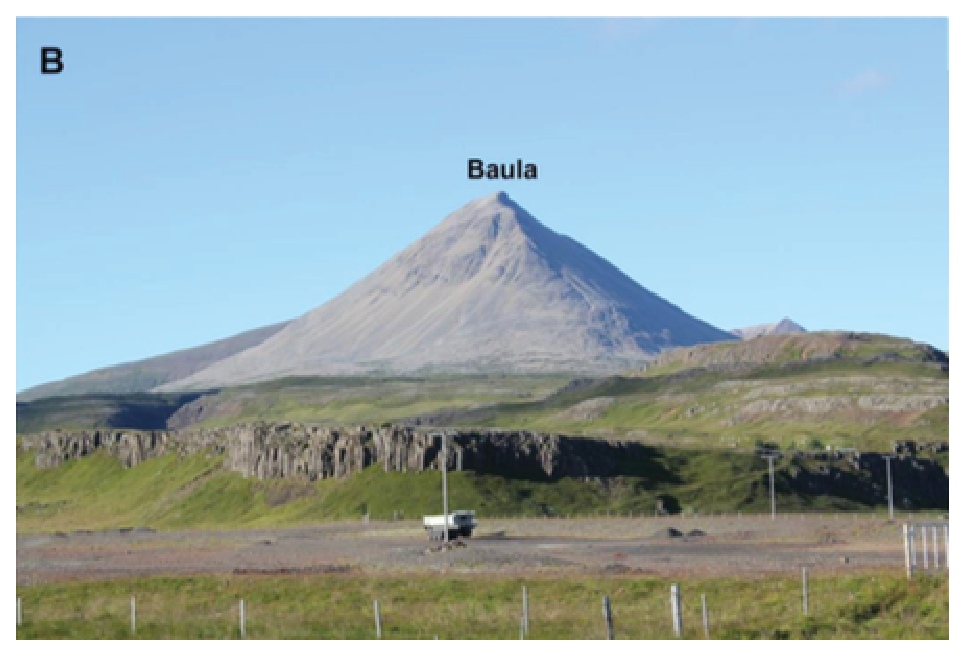
\includegraphics[scale=0.5]{Baula.eps}
    \caption{Felsic laccolith, named Baula, in West Island. Modified
      from \citet{Anonymous:jHnLP36x}.}
    \label{C7-Baula}
  \end{center}
\end{figure}

A  complete description  of the
flow  in  both axysimmetrical  and  cartesian  geometries, along  with
scaling laws  for $h_0(t)$ and  $R(t)$, has already been  described by
\citet{Lister:2013ia}  and   \citet{Anonymous:QWXp_4JV}  respectively.
While the time  dependence of the scaling laws are  similar from those
derived in the bending dominated regime,  the shape of the flow is not
bell-shaped  anymore in  the early  time solution  and shows  somewhat
steeper  edges \citep{Anonymous:QWXp_4JV}.   For instance,  such model
could potentially explain the shape of some felsic laccoliths observed
in Island by \citet{Anonymous:jHnLP36x} (Figure \ref{C7-Baula}).

\subsubsection*{Topography}
\label{sec:topography-1}

As shown in Chapter \ref{C5-chap6},  the topography also imposes large
constrains  on  the  final  morphology of  magmatic  intrusions.   One
interesting avenue for research could be  to model the evolution of an
intrusion  intruding  a  volcanic  edifice.  The  model  developed  in
Chapter \ref{C5-chap6} could  indeed easily be adapted  to account for
the  presence of  a  conic volcanic  edifice on  top  of the  magmatic
intrusion instead  of a depression.   Such model, used  in combination
with  the  geodetic  measurements such  as  Interferometric  Synthetic
Aperture Radar  (InSAR) imaging and  GPS measurements used  to monitor
the deformation on active volcanoes,  could provide a useful framework
to understand  and constrain  the dynamics and  shape of  the volcanic
plumbing systems (Figure \ref{C7-Volcano}).
\begin{figure}[h!]
  \begin{center}
    \graphicspath{ {/Users/thorey/Documents/These/Manuscript/Figure/Chapter7/} }
    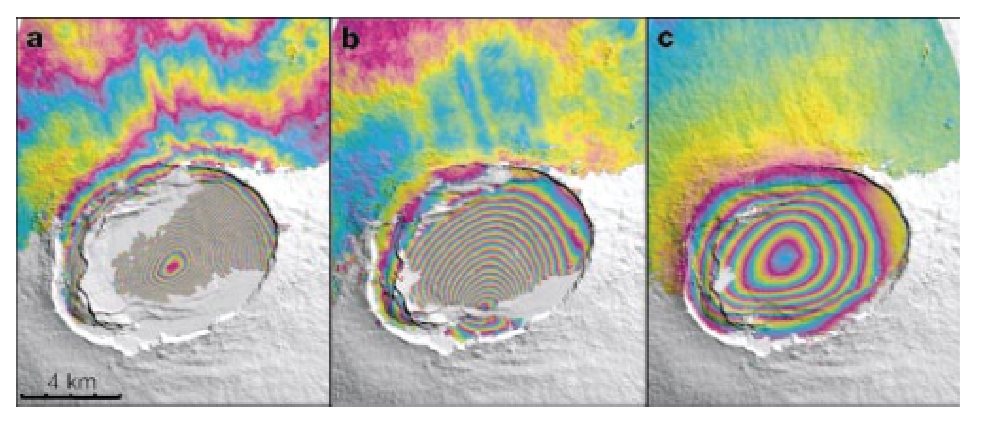
\includegraphics[scale=0.7]{INSAR.eps}
    \caption{Radar  interferograms  of  Sierra Negra  volcano  showing
      uplift during  three time periods.   a, 1992. b, 1997.  c, 1998.
      Each colour cycle represents 5 cm LOS displacement. Modified
      from \citep{Amelung:2000ko}.}
    \label{C7-Volcano}
  \end{center}
\end{figure}

Similar study  could also  be extend to  caldera complexes  which also
often record  ground deformations.   Towards more detailed  studies of
specific area, it could also be interesting to generalize the model in
$3$D. This  will allow to  account directly for the  object topography
one want  to study and hence,  make it easier the  comparison with the
available deformation measurement.


%%% Local Variables:
%%% mode: latex
%%% TeX-master: "../main"
%%% End:

